\documentclass{article}
\usepackage{fixltx2e}
\usepackage{float}
\newcommand{\degree}{\ensuremath{^\circ}}
\usepackage{graphicx}
\usepackage[margin=1.0in]{geometry}



\title{Partial Equilibrium in Mathematica}
\author{Michael Lee, The University of Texas at Austin}

\begin{document}
\maketitle{}

Much of microeconomic analysis is based on the concept of a partial equilibrium. By using computational tools-- such as Mathematica-- we can quickly derive, plot and adapt analytical models of consumer and firm behaviour, and how the intersection of the two fix market equilibrium. 

\newpage

\section{Utility and Production Functions}

The basis of all economic analysis is the consumer and their goal of utility-maximization. The most common numerical repersentation of two-input production and consumer utility are the Cobb-Douglas and Leontief functions. These forms satisfy the following properties depending on if they are used to repersent production or utility, respectively:

\begin{center}
	\begin{enumerate}
		\item monotonicly increasing/decreasing
		\item concave/convex
		\item nonintersecting
	\end{enumerate}
\end{center}

The general Cobb-Douglas function takes the form

$$ Y = L^{\beta}K^{\alpha} $$

Where \emph{Y} is production, \emph{L} is labor, \emph{K} is capital, and $\alpha , \beta$ are the elasticities of labor and capital respectively. The Cobb-Douglass ({\bf Figure 1}) function assumes that continous substitution between goods x\textsubscript{1} and x\textsubscript{2} in production/utility.

\begin{figure}[!ht]
\begin{center}
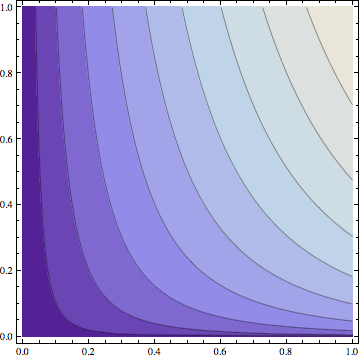
\includegraphics[scale=.5]{Figures/CobbDouglas}
\caption{A Cobb-Douglas Production Function, $\rho = .7$}
\end{center}
\end{figure}

$$ \alpha + \beta = 1 $$
The above equation implies a special conditon when the production function experinces constant returns to scale. \\*
Cobb-Douglas production is a special case of the constant elasticity of substitution (CES) production function as described by Solow (Solow, 1956) when $\lim{\gamma \to 0}$. The two-factor CES function ({\bf Figure 2}) is of the form:

$$
Y = \alpha K^{\gamma} + (1-\alpha) L^{\gamma})^{\frac{1}{\gamma}}
$$

\begin{figure}[!ht]
	\begin{center}
	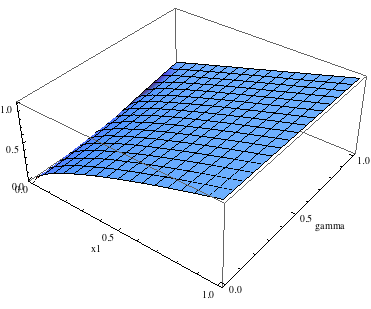
\includegraphics[scale=0.5]{Figures/CES.png}
	\caption{CES Function, $\gamma = [.01,1], x_{1} = [0,1], x_{2} = 1 $}
	\end{center}
\end{figure}
\*


A Leontief function is a special case of a Cobb-Douglas function in which there is no substitutability between goods x\textsubscript{1} and x\textsubscript{2} and thus there exists a predefined proportion of goods x\textsubscript{1} and x\textsubscript{2} used in the production of \emph{Y}. 
$$Y(x_{1}, x_2) = min(c_{1}x_{1}, c_{2}x_{2}) $$

When the proportion 
$$\frac{c_{1}x_{1}}{c_{2}x_{2}} = 1$$
the Leontief has a 45\degree line through the contour plot as seen in {\bf Figure 3}:

\begin{figure}[!ht]
	\begin{center}
	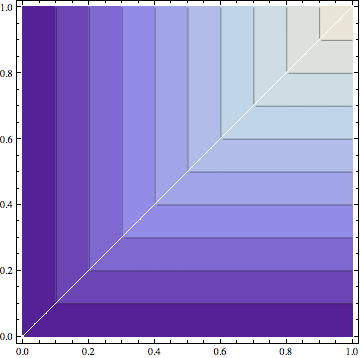
\includegraphics[scale=0.5]{Figures/Leontief.png}
	\caption{A Leontief Production Function}
	\end{center}
\end{figure}


\section{Consumer Theory}
Traditionally, consumer theory is modeled as agents maximizing their utility (strictly a function of consumption, \emph{C}) subject to their budget constraint, (\emph{m}). This implies that given some bundle of goods $x_{1}, x_{2}$ at prices $p_{1}, p_{2}$, the rational consumer will purchase the bundle that maximizes their total utility, \emph{U}. The optimal bundle will allways include an nonzero amount of both goods since utility is subject to the principle of diminishing marginal returns. \*
A Cobb-Douglas utlilty function with elasticities $\alpha$ will take the form:

$$
max U = x_{1}^{\alpha} x_{2}^{1-\alpha}
subject to: m = p_{1}x_{1} + p_{2}x_{2}
$$
\\* \\*
Via logarithims, this equation is equivelent to:

$$
log(U) =  p_{1}log(x_{1}) + p_{2}log(x_{2}) 
$$






\end{document}